\begin{figure*}[t]
    \centering
    \centering
    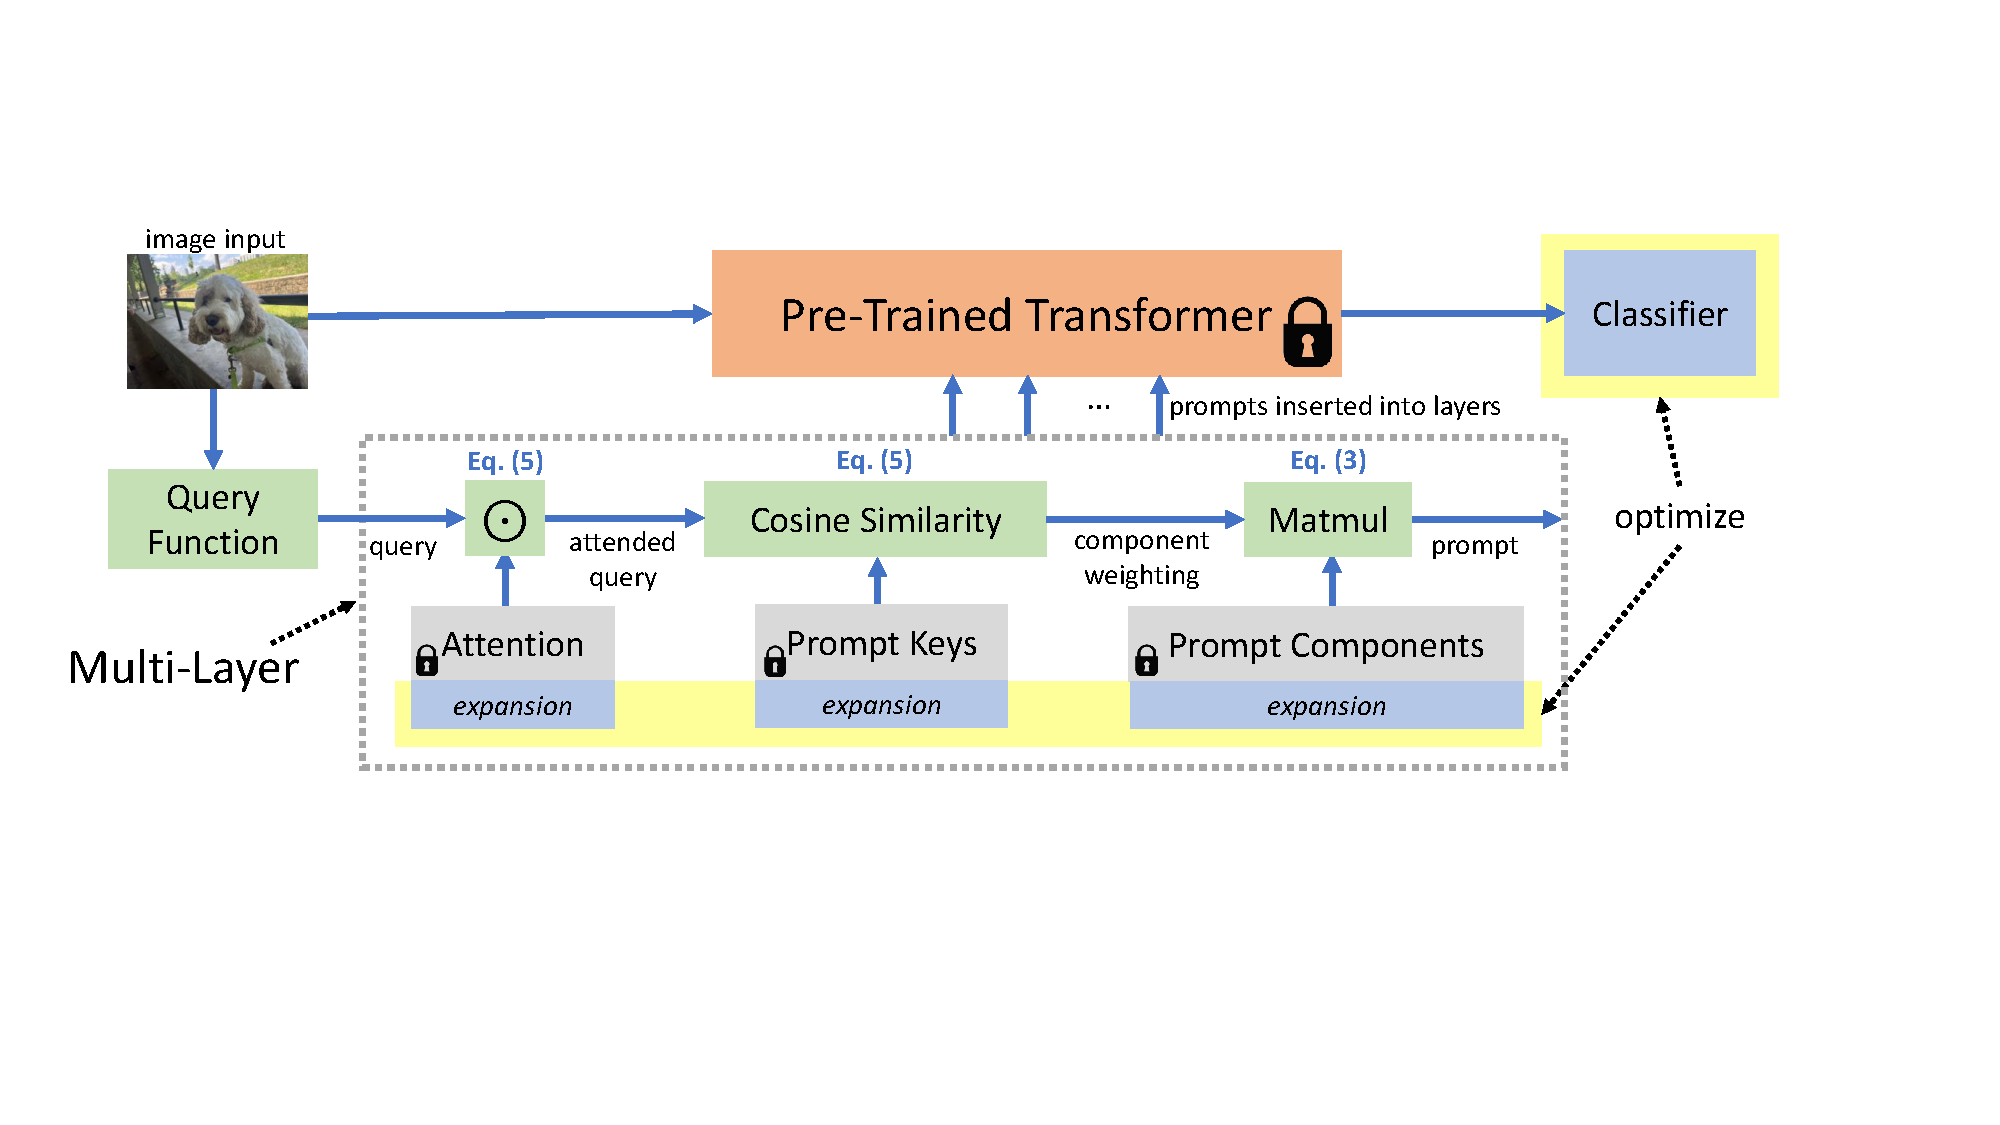
\includegraphics[clip, trim=1.2cm 6cm 3.8cm 3.6cm, width=0.95\textwidth]{figures/source/approach-new.pdf}
    \caption{\textbf{Our CODA-Prompt approach to rehearsal-free continual learning}. An input (e.g., image) is passed through a query function (we use the pretrained ViT encoder) and used for a novel \textbf{attention-based prompt-selection scheme} to produce prompts which are passed to multiple layers of a large-scale, pre-trained transformer. Our method is parameterized by an \emph{expanding} set of small prompt components, with each prompt having a corresponding key and attention vector. Both the input and produced prompts are passed through the transformer and sent to the task head. Only the prompting and task parameters are learned which is \emph{parameter efficient} and no training data is stored for replay which is \emph{memory-efficient and privacy preserving.} \emph{Importantly, our prompt selection scheme can be optimized end-to-end, unlike prior works which have a local similarity-based optimization for key-query matching.}
    }
    \label{fig:method}
    \vspace{-3mm}
\end{figure*}


